%%%%%%%%%%%%%%%%%%%%%%%%%%%%%%%%%%% CABECALHO %%%%%%%%%%%%%%%%%%%%%%%%%%%%%%%%%%%
\documentclass[a4paper]{abnt}

\usepackage[utf8]{inputenc}
\usepackage{csquotes}
\usepackage[brazil]{babel}
\usepackage[T1]{fontenc}
\usepackage[all,defaultlines=2]{nowidow}
\usepackage[multiple]{footmisc}
\usepackage{xcolor,graphicx}
\usepackage[backend=bibtex,backref=true]{biblatex}
\usepackage[colorlinks=true,urlcolor=blue,linkcolor=black,citecolor=red]{hyperref}

\bibliography{projeto}

\author{Igor~Santos}
\title{Projeto~de~TCC - Insert~Coin}

\makeindex
\begin{document}
\maketitle

%%%%%%%%%%%%%%%%%%%%%%%%%%%%%%%%%%%%% INICIO %%%%%%%%%%%%%%%%%%%%%%%%%%%%%%%%%%%%%

\tableofcontents

\chapter{Proposta do Projeto de TCC}

O projeto a ser desenvolvido é um Sistema Pessoal de Planejamento Financeiro, ou de Controle Orçamentário, ou ainda, um Administrador de
Finanças. Seu objetivo é transformar a organização financeira de uma pessoa ou de uma residência, facilitando o manuseio e controle de entrada e saída do dinheiro e das contas bancárias, bem como do cartão de crédito – neste, alterando a forma como o usuário comumente vê o ``plástico''.

Em verdade, o principal diferencial do produto em relação à concorrência atual no mercado será o controle de cartões de crédito. O brasileiro tem o costume de considerar o cartão como um ``gasto'', uma despesa que atrapalha o bom andamento do orçamento familiar, sendo assim um ``mal necessário'' devido aos seus benefícios no adiamento de compras.

O objetivo do \textbf{Insert Coin} nesse sentido é auxiliar o usuário no entendimento dos seus cartões de crédito, e integrá-los ao seu fluxo de caixa normal. Tal fluxo é comumente baseado na entrada de poucas fontes de renda (de alto volume), e a saída em diversas despesas mensais (de volume menor). O cartão de crédito, por ser um concentrador de despesas que adia o pagamento de diversos eventos para um único dia, tende mais confundir do que a ajudar. O usuário precisa compreender bem a dinâmica dos dias de fechamento e de abertura de nova fatura, do ``melhor dia para compra'', o dia do vencimento e quais são os valores possíveis de pagamento – e quais as consequências de não pagar a fatura por completo. Além disso, o lançamento de despesas ocorre com diversos dias de diferença entre o evento e seu aparecimento na fatura parcial. Tudo isso vai muito além do fluxo simples de sua conta-corrente e seu cartão de débito, que consiste em receber o salário do mês, e lançamentos instantâneos do uso do cartão de débito.

%%%%%%%%%%%%%%%%%%%%%%%%%%%%%%%%%%%%%%%%%%%%%%%%%%%%%%%%%%%%%%%%%%%%%%%%%%%%%%%%%%%%%%%%%
\section{O Projeto}

Inicialmente chamado de \textbf{Insert Coin}, ele é principalmente um sistema baseado no lançamento de entradas e saídas de uma ou mais contas de finanças. Ele se assemelha à organização de um Livro-Caixa empresarial, onde o usuário marcará todos os valores recebidos e gastos de uma determinada conta. 

Atualmente existem diversos sistemas no mercado, tanto web quanto móvel, que atendem a esse tipo de usuário, auxiliando na visualização e controle das despesas mensais. Boa parte deles tem o mesmo princípio, inclusive. Portanto, se considerarmos somente esta \emph{feature}, o sistema será pouco diferente do que já existe no mercado e, por exemplo, não incentivará a migração dos usuários de concorrentes para o nosso projeto. Para remediar isso tentaremos inovar na interface e na facilidade de entrada de dados, que é um dos grandes obstáculos para a introdução deste tipo de sistema na rotina do usuário.

Por outro lado, somente um dos sistemas encontrados tenta suprir as peculiaridades do mercado de cartões de crédito nacional, de forma muito vaga e primariamente informativa. O método a ser utilizado aqui é bem mais ativo: ele auxilia o usuário a entender como o cartão de crédito afeta seu fluxo de caixa e insere, como despesas comuns, os eventos nos quais o cartão foi utilizado. O objetivo é evitar a segregação comum que o brasileiro faz em considerar o cartão de crédito com uma mais uma conta/boleto a pagar, como é a eletricidade ou a água da casa. No cartão são feitos gastos assim como ocorrem na conta de débito: lazer, vestuário, transporte, educação, etc. Portanto, porque devemos pensar em ``reduzir os gastos do cartão'' ao invés de ``reduzir os gastos mensais''?

Trabalhando de forma unificada será mais fácil para o usuário compreender o destino do dinheiro daquele mês. Também será possível começar a planejar e organizar metas de redução dos gastos, ou objetivos de economia de forma eficiente e focada. Essa unificação ocorrerá a partir da visualização das despesas daquele mês com relação às entradas; o usuário não precisará se perder em filtros de datas distintos entre a conta-corrente e o cartão de crédito -- que naturalmente possuem fluxos temporais diferenciados. O sistema também evitará a dúvida comum ``será que já posso usar o cartão de crédito?'', auxiliando o usuário a entender as datas importantes de seus cartões, e as inserindo na rotina que ele já conhece e compreende -- a de sua conta corrente e salário.

O que mais cria dúvidas no cartão de crédito é que sua fatura é finalizada cerca de 10 dias antes do dia de pagamento. Aquele período é quando o usuário não está certo de onde as despesas se encaixam melhor: se no mês atual ou no seguinte. Essa confusão se acentua pois as datas da fatura dificilmente encapsulam o período de mês com o qual o usuário está financeiramente acostumado: seu fluxo mensal de entrada do salário. Se ele decide colocar o vencimento do cartão para uma data próxima de seu salário, o fechamento da fatura fica distante do final do mês; se decide fechar a fatura no final do mês, o pagamento fica distante das outras contas que ele comumente paga. E muitas vezes algumas despesas de uma determinada só serão pagas dali a dois meses, o que gera confusão e certa negligência na hora de conferir a origem dos gastos.

A proposta é coletar as datas importantes do cartão e orientar o usuário para que, sempre que possível, a fatura seja paga em cheio no dia do vencimento (em débito automático, por exemplo). Esta é, de acordo com os especialistas da área, a melhor forma de conviver com o cartão, pois não gera juros adicionais em cima do que não foi pago. A partir daí, o usuário terá configurada sua conta-corrente do sistema para que as despesas que ocorrerem no cartão de crédito sejam visualizadas simultaneamente às da conta, no período que corresponda ao pagamento da fatura. Conforme vão surgindo novas despesas no cartão de crédito, o usuário poderá visualizar diretamente seu o impacto no orçamento dos meses seguintes. Também será possível entender de forma prática a fatura do cartão do mês em visualização, juntamente com as contas a serem pagas e as despesas comuns em débito -- afinal de contas, é na conta-corrente que a ação financeira acontece.

%%%%%%%%%%%%%%%%%%%%%%%%%%%%%%%%%%%%%%%%%%%%%%%%%%%%%%%%%%%%%%%%%%%%%%%%%%%%%%%%%%%%%%%%%
\section{Método de Trabalho}
O desenvolvimento do sistema será gerido a partir da área de \emph{Issues} do \textbf{Github}. Lá é possível criar tarefas, categorizar (a partir de \emph{tags}), delegar e ordenar temporalmente. O andamento do projeto será acompanhado a partir de \emph{milestones} configurados no mesmo subsistema, todos com claras datas de finalização.

O \textbf{Github}, além de possuir um subsistema de tarefas, serve principalmente para armazenar na \emph{cloud} um servidor centralizado de \emph{git}. Dessa forma temos automaticamente um sistema eficiente de backup do código do sistema. Ele também participa do ambiente auxiliando a entender o histórico de desenvolvimento no decorrer do tempo; o \emph{git} armazena todas as alterações de código que forem feitas, o que nos ajuda a analisar nossa produtividade e facilmente encontrar os responsáveis por partes do sistema -- útil, por exemplo, quando ocorrer um \emph{bug} inesperado e que precisa ser rapidamente corrigido.

Por fim, para organizar o fluxo de código, será utilizado o \emph{GitFlow}\cite{gitflow} uma metodologia de versionamento que organiza as \emph{tags} de um repositório de forma lógica. A organização precisa desse sistema nos permite criar um fluxo contínuo de \emph{deploys}; podemos configurar nossos servidores de produção para \emph{escutarem} a \emph{tag master} e sempre que houver novos \emph{commits}, eles podem importar a nova versão - isso é feito a partir de \emph{git hooks}, ou automaticamente por alguns sistemas de \emph{PaaS}.

\begin{figure}
	\centering
	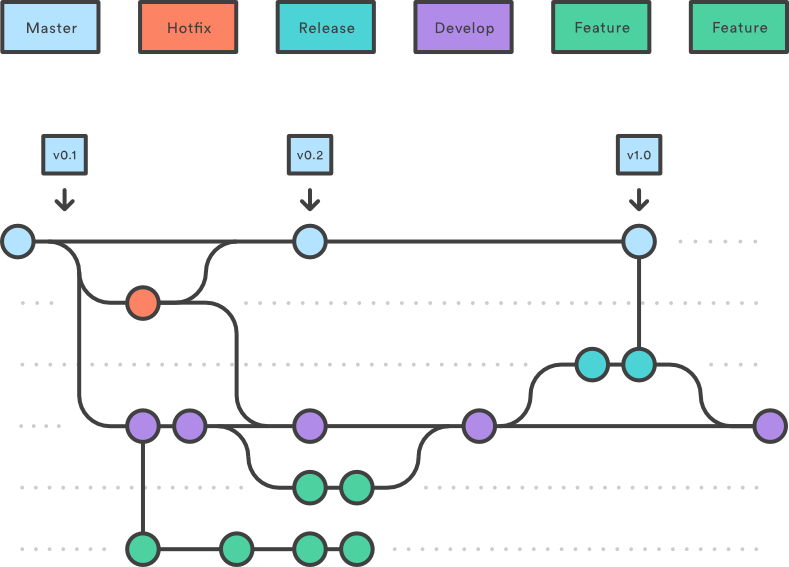
\includegraphics[scale=0.65]{img/gitflow.png}
	\caption{Exemplo de como \emph{GitFlow} funciona, exibindo os diversos \emph{branches} da metodologia.}
\end{figure}

%%%%%%%%%%%%%%%%%%%%%%%%%%%%%%%%%%%%%%%%%%%%%%%%%%%%%%%%%%%%%%%%%%%%%%%%%%%%%%%%%%%%%%%%%
\section{Previsão de Alocação de Recursos}

\subsection*{Recursos Humanos}
\begin{itemize}
	\item 1 Analista de Sistemas Sênior;
	\item 1 Designer multi-plataforma (\textit{web} e móvel);\footnotemark
	\item 1 Analista de marketing \emph{freelancer} (para o marketing inicial do produto; futuramente, integrará a equipe permanente).
\end{itemize}

\subsection*{Recursos Materiais}
\begin{itemize}
	\item Instâncias no \emph{Heroku} (é possível começar com pouco e expandir facilmente no futuro\cite{heroku}) com as seguintes configurações:
	\begin{itemize}
		\item \emph{Dynos web} (máquinas que processam \emph{requests} web) rodando \textbf{PHP 5.5};
		\item \emph{Dynos de background} 
		\item Servidor \textbf{PostgreSQL}, também facilmente escalável e seguro\cite{heroku-pgsql};
		\item Servidor de Cache HTTP \textbf{Varnish} em cada \emph{dyno} para otimizar os requests estáticos ou repetidos;
	\end{itemize}
	
	\item Os seguintes add-ons a partir da plataforma do \emph{Heroku}:
	\begin{itemize}
		\item Servidor de \emph{Memcache} \textbf{MemCachier} para caches temporários de aplicação;
		\item \textbf{Mandrill by MailChimp} para envio de e-mails de lembretes;
		\item \textbf{NewRelic} para monitoria da performance da aplicação e do banco de dados;
		\item \textbf{Rollbar} para monitoria de erros nas aplicações.
	\end{itemize}
\end{itemize}

%%%%%%%%%%%%%%%%%%%%%%%%%%%%%%%%%%%%%%%%%%%%%%%%%%%%%%%%%%%%%%%%%%%%%%%%%%%%%%%%%%%%%%%%%
\section{Cronograma de Trabalho}

%=======================================
%
%    [TODO] Criar gráfico de Gantt
%
%=======================================

%%%%%%%%%%%%%%%%%%%%%%%%%%%%%%%%%%%%%%%%%%%%%%%%%%%%%%%%%%%%%%%%%%%%%%%%%%%%%%%%%%%%%%%%%
\chapter{A Empresa e o Negócio}
O objetivo do projeto é entrar num mercado já saturado de aplicativos similares com uma lista de diferenciais para atrair os consumidores que ainda não utilizam sistemas automatizados de gestão financeira ou se sentem insatisfeitos com as soluções que usam atualmente. Para isso, a equipe de desenvolvimento focará numa usabilidade simples e no menor atrito possível para entrada de novos lançamentos. E, por outro lado, o diferencial em funcionalidades terá como carro-chefe o tratamento do cartão de crédito de forma diferenciada das contas corrente e poupança, como nenhum aplicativo do mercado faz atualmente.

Todos os responsáveis pelo projeto tem larga experiência prática em diversos métodos de organização financeira e são usuários de diferentes sistemas do mercado. Portanto, todos são hábeis de opinar e desenvolver o projeto da melhor forma possível, com boas sugestões de funcionalidades e ao mesmo tempo evitando os erros (de acordo com nosso ponto de vista) já cometidos pela concorrência.

O sistema funcionará no modo \textit{freemium}, onde os usuários terão acesso a um grupo limitado de funcionalidades e precisarão pagar mensalmente caso desejem utilizar as funções avançadas. A lista final do que será de uso gratuito e do que será pago só será de fato conhecida quando o escopo do projeto for fechado; no entanto, segue um exemplo de algumas funcionalidades mais complexas e que fazem sentido entrar na lista \textit{premium}:
\begin{itemize}
	\item Gráficos e análises financeiras sobre os gastos mensais e anuais
	\item Ter mais de duas contas (sendo uma corrente e uma poupança\footnote{Isso caracterizaria um usuário avançado, visto que o caso mais comum é o brasileiro ter uma conta-corrente onde recebe seu pagamento (ou uma conta-salário e uma corrente), e talvez uma poupança onde ele guarda suas economias, e diversos cartões de crédito.})
	\item A possibilidade de planejar o pagamento parcial de uma fatura de cartão de crédito
	\item Uso do aplicativo móvel em modo offline, permitindo sincronia de dados quando o aparelho entrar numa conexão \textit{WiFi}
	\item Integração entre mais de um usuário numa mesma conta -- por exemplo, um casal usando o mesmo sistema a partir de dois \textit{logins} diferentes
\end{itemize}
 
%%%%%%%%%%%%%%%%%%%%%%%%%%%%%%%%%%%%%%%%%%%%%%%%%%%%%%%%%%%%%%%%%%%%%%%%%%%%%%%%%%%%%%%%%
\section{Histórico}
A empresa responsável pelo \textbf{Insert Coin} foi criada especialmente para o projeto, a partir da sintonia de ideias entre o Analista e o Designer a cargo. A ideia surgiu quando o Analista se sentia insatisfeito com o sistema de gestão que utilizava e não conseguiu encontrar substituto eficaz no mercado. O que mais lhe incomodava era não ser fácil controlar os gastos em cartão de crédito, pois as aplicações disponíveis só possuíam a distinção entre múltiplas ``contas'', e o ciclo de vida de uma fatura acabava por ficar misturado com o fluxo de caixa da conta-corrente, por exemplo. A ideia foi fomentada aos poucos e então surgiu a oportunidade de, junto ao seu colega de graduação, iniciar a estruturação e o desenvolvimento do projeto.

%%%%%%%%%%%%%%%%%%%%%%%%%%%%%%%%%%%%%%%%%%%%%%%%%%%%%%%%%%%%%%%%%%%%%%%%%%%%%%%%%%%%%%%%%
\section{Mercado Consumidor}
\label{sec:mercado}
O público-alvo do projeto tem uma ou mais de cada uma das seguintes características:
\begin{enumerate}
	\item Em relação às suas finanças:
		\begin{itemize}
			\item Nunca se informou sobre educação financeira antes, mas começou a se interessar sobre o assunto;
			\item Já tem um certo nível de organização financeira, mas ela é falha ou rudimentar;
			\item Tem suas planilhas eletrônicas financeiras, mas são complexas de usar e engessadas;
			\item Encontra problemas de se manter no azul, e está em busca de de soluções para sua falta de controle;
		\end{itemize}
	\item Em relação à tecnologia:
		\begin{itemize}
			\item Possui um smartphone e tem um uso aceitável do mesmo, mas não usa o computador com frequência;
			\item Possui ou não um smartphone e se sente confortável navegando na Internet;
			\item Possui ou não um smartphone e utiliza planilhas eletrônicas para controlar suas finanças;
		\end{itemize}
\end{enumerate}

Ou seja, nosso principal mercado consumidor tem algum contato com tecnologia e se sente confortável a usá-la, seja no computador ou num dispositivo móvel, e tem algum interesse em educação e organização financeira, seja por dificuldades anteriores ou por puro interesse pessoal.

%%%%%%%%%%%%%%%%%%%%%%%%%%%%%%%%%%%%%%%%%%%%%%%%%%%%%%%%%%%%%%%%%%%%%%%%%%%%%%%%%%%%%%%%%
\section{Concorrência}
Atualmente no mercado há diversas empresas focadas em produtos similaeres ao que propomos neste projeto. No entanto, foi identificado que nenhum deles oferece todas as funcionalidades que planejamos implementar, o que significa que, após o lançamento vamos estar à frente da concorrência e aptos a conquistar novos clientes, sejam estes experientes em outros produtos ou interessados em experimentar algo novo.\\
Listamos aqui as principais empresas concorrentes até o momento:

\begin{center}
	\begin{tabular}{|c|c|c|}
		\hline 
		\textbf{Granatum} & \textbf{Organizz}e & \textbf{Mint (americano)} \\\hline 
		Yupee & MyFreeComm Finance & Manubia \\\hline 
		Monefy & \multicolumn{2}{c|}{\emph{Outros aplicativos móveis similares}} \\\hline 
	\end{tabular}
\end{center}

Foi notado que algumas empresas possuem parceria com algumas instituições bancárias, o que em tese poderia trazer mais clientes destes bancos aos seus aplicativos. No entanto, não há notícia de divulgação destes sistemas dentro das agências ou em outros veículos relacionados aos bancos. Isso nos leva a crer que a parceria foi criada para iniciar um processo de integração bancária, mas por motivos alheios ao conhecimento geral, tal integração não evoluiu com outros bancos. 
A única exceção a essa regra é o \emph{Mint}, mas que não representa concorrência direta por n\~ao fazer parte do mercado nacional. Apesar disso, ele é listado aqui para servir de exemplo sobre como a vida do usuário pode ser facilitada; o sistema do \emph{Mint} possui integração com uma longa, longa lista de instituições financeiras dos Estados Unidos e do Canadá. Isso permite que o usuário não precise criar novas entradas manualmente para se organizar -- o sistema busca, em \emph{background}, as informações diretamente com os bancos e administradoras de cart\~oes.

%%%%%%%%%%%%%%%%%%%%%%%%%%%%%%%%%%%%%%%%%%%%%%%%%%%%%%%%%%%%%%%%%%%%%%%%%%%%%%%%%%%%%%%%%
\section{Premissas e Restrições ao Projeto}
Os principais objetivos do projeto, a nível de funcionalidades, seguem abaixo. A lista está ordenada aproximadamente por prioridade de implementaç\~ao, e os itens enfatizados provavelmente far\~ao parte da lista de recursos avançados, oferecidos somente aos usuários \emph{premium}:
\begin{enumerate}
	\item Lançamento de despesas diárias e visualizaç\~ao em estilo de planilha;
	\item Divis\~ao em contas distintas, com tratamento especial para cart\~oes de crédito;
	\item Categorias personalizadas de lançamentos, com cores para facilitar identificaç\~ao;
	\item Categorizaç\~ao opcional por meio de pagamento (boleto, cart\~ao, transfer\^encia, etc);
	\item Inclus\~ao de lançamentos parcelados e periódicos;
	\item Filtragem de despesas por m\^es ou período de livre escolha;
	\item \emph{Acompanhamento de metas de valores mensais para categorias definidas;}
	\item Planejamento avançado dos próximos meses, a partir dos lançamentos futuros e das metas pretendidas;
	\item Tela inicial personalizável, com blocos de resumos, lançamento rápido, saldos, etc;
	\item Aplicativo móvel, para facilitar a visualizaç\~ao do orçamento e o registro imediato de despesas feitas na rua. Ele precisará de uma interface inovadora na tela de novo lançamento, de modo a diminuir ao máximo a quantidade de interaç\~oes necessárias -- dessa forma, reduzindo o atrito dessa aç\~ao frequente para o usuário;
	\item Notificaç\~oes de lançamentos a vencer via e-mail e no aplicativo móvel;
	\item \emph{Resumo histórico, para um entendimento mais amplo da vida financeira do usuário;}
	\item \emph{Gráficos de análise financeira por período, categorias, e contas;}
	\item Integraç\~ao com sistema de relatórios de erros e pedidos de novos recursos pelos usuários;
	\item Sistema de importaç\~ao simplificada dos arquivos exportados pelos principais bancos;
	\item \emph{Leitor OCR\footnote{Reconhecimento Ótico de Caracteres: tecnologia que traduz uma imagem de texto em palavras} inteligente, para capturar informaç\~oes de um novo lançamento a partir de uma foto do comprovante de crédito/débito, tirada com o celular};
	\item Equiparaç\~ao de funcionalidades do sistema web com o aplicativo móvel, de forma que os usuários possam ter liberdade total de usar somente o dispositivo móvel se preferirem;
	\item \emph{Integraç\~ao com sistemas bancários}
\end{enumerate}

Esta lista de funcionalidades previstas para o sistema n\~ao é definitiva, o que significa que no decorrer do projeto há a possibilidade de novas ideias surgirem e serem realocadas no planejamento, de acordo com a demanda. Além disso, devido ao seu tamanho, foi decidido que os recursos numerados de 10 em diante ser\~ao desenvolvidos numa fase futura do sistema -- portanto, fora do escopo deste Trabalho de Conclus\~ao de Curso.

Dito isto, é notável que a maior restriç\~ao para o projeto será o fator temporal. O objetivo é que o \textbf{Insert Coin} seja um sistema em eterno andamento, com o lançamento gradual de novas funcionalidades. Esse comportamento ajuda a manter os usuários fiéis e um fluxo contínuo de novos clientes. A fidelidade se dará pelos seguintes pontos:
\begin{itemize}
	\item Saber que os problemas encontrados ser\~ao resolvidos em breve;
	\item O usuário será sempre o foco da empresa, que estará sempre adicionando novos recursos para o melhor aproveitamento de suas informaç\~oes financeiras;
	\item Ele poderá participar indiretamente do desenvolvimento do produto, através do \emph{feedback} interativo, reportando problemas encontrados e sugerindo novas funcionalidades que julgar relevante para si.
\end{itemize}

%%%%%%%%%%%%%%%%%%%%%%%%%%%%%%%%%%%%%%%%%%%%%%%%%%%%%%%%%%%%%%%%%%%%%%%%%%%%%%%%%%%%%%%%%
\chapter{Os Sistemas Atuais}

%%%%%%%%%%%%%%%%%%%%%%%%%%%%%%%%%%%%%%%%%%%%%%%%%%%%%%%%%%%%%%%%%%%%%%%%%%%%%%%%%%%%%%%%%
\section{Principais Concorrentes}
Para um melhor entendimento do mercado atual, é necessário que analisemos em maior profundidade os principais sistemas com os quais vamos concorrer por público. É essencial absorver as funcionalidades que s\~ao o carro-chefe de cada um destes produtos, para que seja possível balancear nosso projeto e fazer frente ao mercado corrente:

\begin{description}
	\item[Organizze] Sistema mais completo atualmente para o usuário final. Possui diversas contas e tratamento especial para cart\~oes, mas tal diferenciaç\~ao é básica, se restringindo a dividir os lançamentos do cart\~ao em faturas. Possui também metas, que n\~ao contribuem para o planejamento mensal ou futuro. Também conta com lançamentos repetidos e parcelados, além de um aplicativo para avaliaç\~ao dos lançamentos do mês e criaç\~ao de novos. O sistema possui uma interface clean e bem espaçada, o que pode incomodar alguns usuários que est\~ao acostumados com maior volume de informaç\~oes (vindos de outros sistemas ou de planilhas, por exemplo).
	
	\item[Granatum] Segundo maior concorrente, apesar de ter foco maior no público corporativo. O sistema de gest\~ao pessoal est\'a abandonado h\'a v\'arios anos, n\~ao recebendo sequer uma melhoria ou correç\~ao. No entanto, gradualmente a vers\~ao empresarial tem sido renovada, ent\~ao talvez o plano pessoal seja atualizado tamb\'em -- ou descontinuado. Em matéria de recursos, é muito similar ao \emph{Organizze}, exceto pelo aplicativo móvel ter sido lançado h\'a pouco tempo, e n\~ao funcionar corretamente com contas pessoais. Também n\~ao possui tratamento especial das despesas de cart\~ao de crédito, e sua listagem de lançamentos se assemelha mais com uma planilha eletr\^onica do que o outro concorrente.
	
	\item[Mint] ``Concorrente'' americano. Líder de mercado da América do Norte, principalmente nos Estados Unidos, onde já se consolidou como ferramenta de gest\~ao financeira pessoal há muitos anos. O principal diferencial é a habilidade de importar automaticamente e sem intervenç\~ao todos os lançamentos ocorridos nas contas bancárias e seus cart\~oes, dos mais diversos bancos. Isso permite ao usuário somente categorizar e organizar as despesas, facilitando bastante a tarefa de analisar os gastos e sua saúde financeira de modo geral. No entanto, por causa de sua natureza focada no histórico bancário, o sistema n\~ao permite o planejamento futuro a partir de previ\~oes de gastos e lançamentos adiantados, o que reduz bastante os benefícios para o usuário final. Suas integraç\~oes estreitas permitem a monetizaç\~ao facilitada, oferecendo ao cliente diversos outros produtos, como: cart\~ao com taxas mais em conta no caso de serem identificadas altas taxas nos atuais; previd\^encia privada baseada nas economias passadas; avisos sobre taxas inesperadas cobradas pelos bancos; dentre outros.
	
	\item[Monefy] Um dos aplicativos móveis mais inovadores do mercado. Possui uma interface diferente para lançamento de despesas e receitas, que foca na categorizaç\~ao simplificada a partir de ícones. O aplicativo também possui uma calculadora na tela de valor e descriç\~ao, o que facilita a atualizaç\~ao de um lançamento anterior ou o agrupamento de despesas numa só entrada. Ele também possui a opç\~ao de alterar a moeda corrente do sistema, apesar de n\~ao permitir moedas distintas para cada conta. Sua tela principal consiste de um gráfico que facilmente demonstra ao usuário quais s\~ao suas principais fontes de despesas -- mas fora isso, n\~ao colabora com outros métodos de análise. Há também um widget, que pode até mesmo ser usado diretamente da tela de bloqueio do telefone.
\end{description}

%%%%%%%%%%%%%%%%%%%%%%%%%%%%%%%%%%%%%%%%%%%%%%%%%%%%%%%%%%%%%%%%%%%%%%%%%%%%%%%%%%%%%%%%%
\section{Outros Sistemas}
Além dos sistemas digitais, também enfrentaremos um comportamento comum de novos usuários: o receio de migrar de plataforma. Para lidar com a migraç\~ao de outros sistemas, o usuário poderá importar seus dados, caso o outro suporte a exportaç\~ao também. No entanto, o maior receio poderá ser a mudança para um sistema informatizado e \emph{online} a partir de uma organizaç\~ao tradicionalmente analógica. Portanto, vamos tentar entender as principais vantagens e desvantagens dos sistemas n\~ao-inteligentes mais comuns:

\begin{description}
	\item[Caderno de anotaç\~oes / agenda] O tradicional par \emph{papel \& caneta} ganha o cliente no quesito facilidade, pois é extremamente prático fazer uma nova linha para cada nova despesa. No entanto, o caderno perde e muito quando o usuário deseja: identificar uma despesa antiga; fazer correç\~oes; planejamento do futuro; fazer análises; dentre outros. Em todos estes pontos a interface digital poderá facilitar, e será necessário demonstrar isso para poder convencer este tipo de usuário a migrar.
	
	\item[Planilhas eletrônicas] O meio de entrada mais comum para a informatizaç\~ao das finanças de certo grupo de usuários. Ganha na versatilidade e adaptaç\~ao ao modo de pensar de cada pessoa, e também na facilidade de acesso, visto que normalmente n\~ao depende de internet para ser utilizado -- apesar de perder em portabilidade. No entanto, a fluidez de uso do sistema é deficiente, visto que será necessário o conhecimento avançado deste tipo de aplicativo para muitos recursos além do básico da gest\~ao financeira, como resumos, análise de longos períodos, ou visualizaç\~oes gráficas. Além do mais, o usuário sempre corre o risco de ter danos em seu computador e n\~ao possuir um backup recente dos arquivos. Para este tipo de usuário precisaremos indicar as vantagens de um sistema mais robusto e online.
\end{description}

%%%%%%%%%%%%%%%%%%%%%%%%%%%%%%%%%%%%%%%%%%%%%%%%%%%%%%%%%%%%%%%%%%%%%%%%%%%%%%%%%%%%%%%%%
\section{Motivaç\~oes para o Novo Sistema}
Como indicado na seç\~ao \ref{sec:mercado}, há diversos tipos de usuários que poder\~ao se interessar por um sistema como o \textbf{Insert Coin}. Para trazê-los ao sistema, será necessário chamar a atenç\~ao de cada um deles de forma diferente. Segue aqui uma sugest\~ao de bons motivos para a migraç\~ao, ou mesmo para iniciarem seu controle financeiro pelo projeto:

\begin{description}
	\item[Controle] O sistema dará nas m\~aos do usuário a possibilidade de ter o controle total sobre seu dinheiro, tendo conhecimento do que entra e sai de suas contas;
	\item[Organizaç\~ao] Visualizaç\~ao dos dados de entradas e saídas dados em diferentes formatos e granularidades;
	\item[Simplicidade] A facilidade de uso permitirá ao usuário usufruir destas qualidades sem sofrer com a perda de tempo, que normalmente ocorre em sistemas robustos e complexos;
	\item[Praticidade] Uma vers\~ao móvel simples do sistema é essencial para diminuir o atrito de uma atividade rotineira como o lançamento de despesas cotidianas;
	\item[Futuro] A visualizaç\~ao condensada do passado e as possibilidades de metas e lançamentos futuros levará o usuário à previs\~ao de sua saúde financeira; isso permitirá maior conforto e liberdade em compras parceladas, ou o planejamento de sonhos como a compra da casa própria, um carro novo, ou uma grande viagem.
\end{description}

%%%%%%%%%%%%%%%%%%%%%%%%%%%%%%%%%%%%%%%%%%%%%%%%%%%%%%%%%%%%%%%%%%%%%%%%%%%%%%%%%%%%%%%%%
\subsection{Problemas dos Sistemas Atuais}
Nenhum sistema é perfeito; a principal chance de chegar ao mercado com um produto de sucesso é explorando as fraquezas dos concorrentes, e construindo em cima destes conceitos para que n\~ao sejam repetidos os mesmos erros.

Foi possível identificar, em diversos produtos menores do mercado, características similares de complexidade desnecessária para o usuário mediano, por exemplo. Esse tipo de comportamento afasta o usuário mais leigo, ao invés de estimulá-lo a uma vida financeira mais saudável.

Outra quest\~ao recorrente nas conversas com diversos usuários foi a ``preguiça'' gerada pelo trabalho rotineiro de controle das despesas. A maioria dos sistemas online exige alguns cliques até chegar à tela de novo lançamento, o que dificulta bastante o uso frequente. Os aplicativos móveis ganham nesse quesito, por estarem ``sempre \`a m\~ao'', sendo normalmente de uso mais pr\'atico. Por outro lado, h\'a poucas soluç~oes integradas no mercado, que unam a versatilidade de um sistema móvel com o poder de análise de um sistema \emph{web/desktop}.

%%%%%%%%%%%%%%%%%%%%%%%%%%%%%%%%%%%%%%%%%%%%%%%%%%%%%%%%%%%%%%%%%%%%%%%%%%%%%%%%%%%%%%%%%
\subsection{Situação Desejada}
O objetivo final do projeto é dar ao usuário uma vida financeira mais estável e próspera, lhe permitindo visualizar oportunidades de economia que antes não eram visíveis. Dessa forma, o cliente poderá planejar e alcançar sonhos que antes eram muito distantes, a partir da organização de metas de gastos e de economias. 

Isso poderá ser atingido com um sistema integrado que possibilite a análise de dados e histórico numa interface simples de entender, aliada a um aplicativo móvel que torne prática e rápida a tarefa cotidiana de acompanhamento financeiro. 

%%%%%%%%%%%%%%%%%%%%%%%%%%%%%%%%%%%%%%%%%%%%%%%%%%%%%%%%%%%%%%%%%%%%%%%%%%%%%%%%%%%%%%%%%
\chapter{O Sistema Proposto}
Para uma etapa de desenvolvimento fluida e para o continuo aprimoramento do sistema, se faz necessária a documentação técnica do mesmo. É de suma importância que estas informações se mantenham ``vivas'' assim como a própria implementação, de modo que sempre possamos nos apoiar numa documentação sólida e de fácil entendimento sempre que surgirem dúvidas ou para subdividir as tarefas de desenvolvimento em passos lógicos. 

%%%%%%%%%%%%%%%%%%%%%%%%%%%%%%%%%%%%%%%%%%%%%%%%%%%%%%%%%%%%%%%%%%%%%%%%%%%%%%%%%%%%%%%%%
\section{Requisitos do Sistema}
Para que o \textbf{Insert Coin} atinja de forma eficaz seus objetivos será necessário cumprir os requisitos técnicos descritos a seguir. 

%=======================================
%
%    [TODO] Revisar requisitos para
%           dividir entre funcionais
%           e não-funcionais
%
%=======================================

\subsection{Design}
\begin{itemize} 
	\item Interface limpa e simplificada, de modo a não confundir o usuário desacostumado;
	\item Categorias de fácil identificação visual;
\end{itemize}

\subsection{Implementação}
\begin{itemize} 
	\item Certificado de segurança SSL para as comunicações de todos os servidores HTTP (tanto de API quanto de aplicação), em todas as aplicações e subsistemas;
\end{itemize}

\subsubsection{Servidor REST}
\begin{itemize} 
	\item Autenticação via \emph{Auth header}\footnote{Método de autenticação padrão do HTTP.}, e \emph{fallback} com cookie, para facilitar a implementação de diversos tipos de clientes\cite{auth};
	\item Respostas curtas e compactadas com Gzip, para economia de dados e redução da latência no uso móvel;
	\item Documentação da API extensa e de rápido entendimento;
	\item Extensa suíte de testes para garantir que os aplicativos não falharão por causa da API;
\end{itemize}

\subsubsection{Aplicativo Web}
\begin{itemize}
	\item Layout fluido e responsivo, que se adapte a diversos formatos de telas, como celulares, tablets, e telas largas ou estreitas\footnote{Uma visualização mais estreita do sistema, principalmente nas telas de lançamentos, pode ser útil em atividades comparativas --- quando acessando lado a lado com o histórico bancário, por exemplo} no computador;
	\item Vis\~oes detalhadas dos dados, com todas as opç\~oes oferecidas para históricos, resumos e gráficos;
\end{itemize}

\subsubsection{Aplicativo Móvel}
\begin{itemize}
	\item Suporte a diversas plataformas (mínimo: iOS e Android), para evitar a perda de usuários por causa do ambiente;
	\item Login automático e silencioso após a autenticaç\~ao inicial;
	\item Funcionamento \emph{offline} sem afetar a usabilidade ou performance;
	\item Sincronizaç\~ao de dados manual e automática em \emph{background} (quando encontrar uma conex\~ao WiFi, ou via dados móveis também, caso o usuário deseje);
	\item Funcionalidades básicas de análise, como históricos, resumos, filtros e alguns gráficos;
\end{itemize}
		

%%%%%%%%%%%%%%%%%%%%%%%%%%%%%%%%%%%%%%%%%%%%%%%%%%%%%%%%%%%%%%%%%%%%%%%%%%%%%%%%%%%%%%%%%
\begin{figure}
	\section{Casos de Uso}
	\centering
	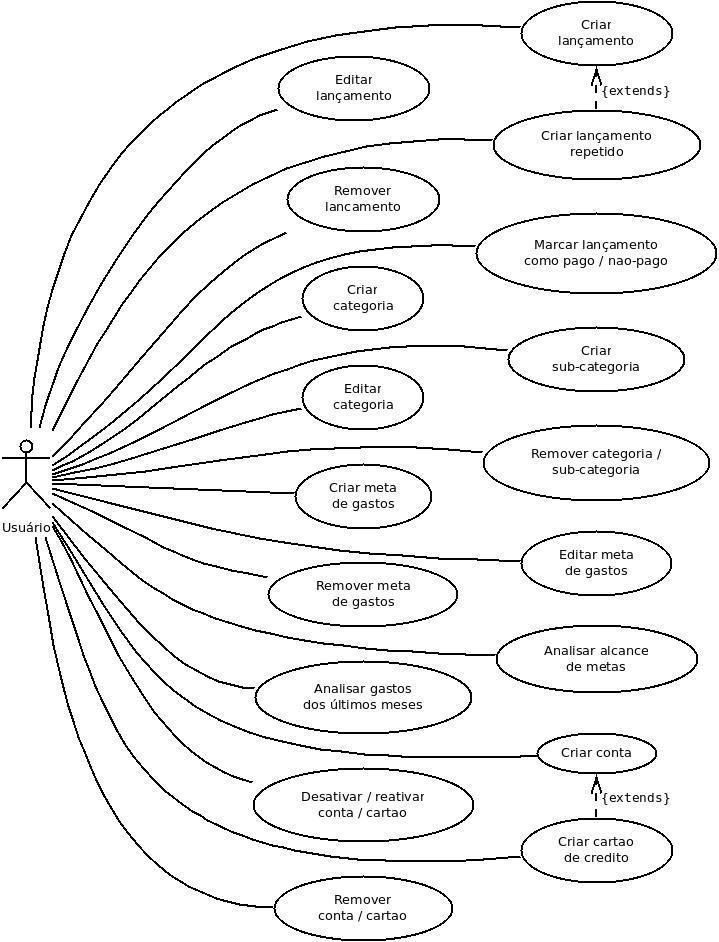
\includegraphics[scale=0.6]{diagramas/casos-de-uso.jpg}
	\caption{Diagrama de Casos de Uso}
\end{figure}


%%%%%%%%%%%%%%%%%%%%%%%%%%%%%%%%%%%%%%%%%%%%%%%%%%%%%%%%%%%%%%%%%%%%%%%%%%%%%%%%%%%%%%%%%
\subsection{Especificações}

%=======================================
%
%    [TODO] Especificar casos de uso
%
%=======================================

\subsubsection{Criar Lançamento}
\subsubsection{Criar Lançamento Repetido}
\subsubsection{Editar Lançamento}
\subsubsection{Remover Lançamento}
\subsubsection{Marcar Lançamento como Pago / não-pago}
\subsubsection{Criar Categoria}
\subsubsection{Criar Sub-categoria}
\subsubsection{Editar Categoria}
\subsubsection{Remover Categoria / Sub-categoria}
\subsubsection{Criar Meta de Gastos}
\subsubsection{Editar Meta de Gastos}
\subsubsection{Remover Meta de Gastos}
\subsubsection{Analisar Alcance de Metas}
\subsubsection{Analisar Gastos dos Últimos Meses}
\subsubsection{Criar Conta}
\subsubsection{Criar Cart\~ao de Crédito}
\subsubsection{Desativar / reativar conta / cartão}
\subsubsection{Remover conta / cartão}

%%%%%%%%%%%%%%%%%%%%%%%%%%%%%%%%%%%%%%%%%%%%%%%%%%%%%%%%%%%%%%%%%%%%%%%%%%%%%%%%%%%%%%%%%
\pagebreak
\section{Diagrama de Topologia}
\begin{figure}[!h]
	\centering
	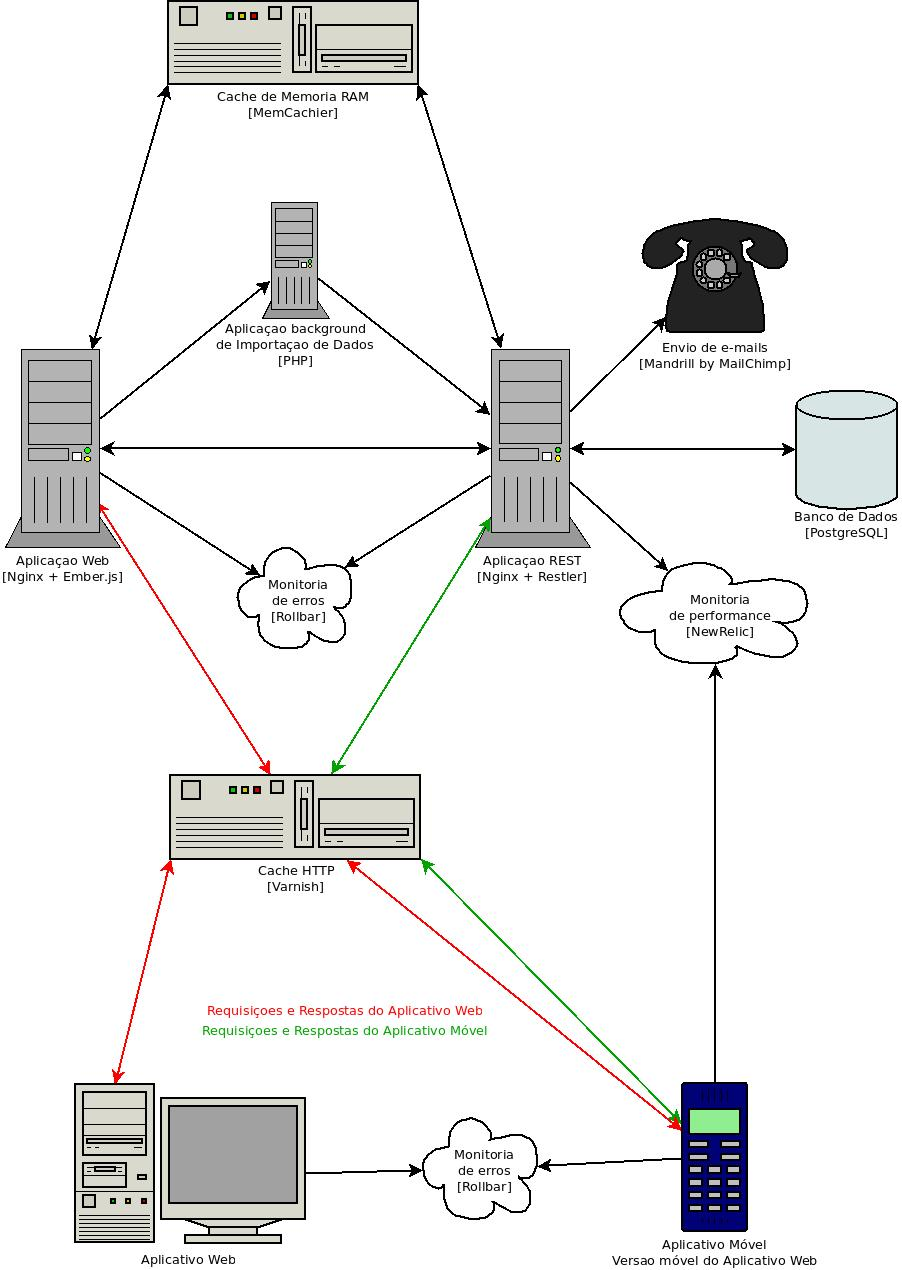
\includegraphics[scale=0.48]{diagramas/topologia.jpg}
	\caption{Diagrama de Topologia, indicando os diversos servidores de aplicaç\~ao, de cache, serviços adicionais e o fluxo de comunicaç\~ao com os aplicativos-cliente}
\end{figure}

%%%%%%%%%%%%%%%%%%%%%%%%%%%%%%%%%%%%%%%%%%%%%%%%%%%%%%%%%%%%%%%%%%%%%%%%%%%%%%%%%%%%%%%%%
\section{Modelo Conceitual de Classes}
Neste diagrama descrevemos as principais classes do Servidor REST do projeto. É possível notar que as classes refletem em boa parte o Modelo de Dados (proposto na seção seguinte, \ref{sec:mod_dados}). Isso ocorre pois o servidor funcionará, principalmente, como um sistema de banco de dados de forma simplificada, armazenando todas as regras de negócio e, em alguns casos, expondo métodos mais inteligentes e ágeis que o tradicional \emph{CRUD}. 

O método de espelhamento do banco proporcionará aos aplicativos a maior liberdade possível para serem desenvolvidos e se adaptarem aos seus ambientes, ao invés de se adaptarem ao modelo de dados proposto por um servidor mais enxuto. No entanto, ao mesmo tempo ele garante os requisitos básicos de segurança e funcionalidades, por implementar todas as regras de negócio relacionadas aos dados conjuntamente com os mesmos.

Todos os métodos demonstrados por estas classes são baseados no formato da biblioteca \emph{Restler}, que interpreta classes gerais (não-necessariamente com uma hierarquia em comum) e abre seus métodos públicos num \emph{endpoint HTTP}. Dessa forma, as classes se tornam \emph{recursos}, e os métodos possuem nomes dos \emph{verbos HTTP}; opcionalmente, também são acompanhados de um sufixo que indica uma ação mais específica dentro daquele recurso.

\begin{table}[hb]
\begin{flushleft}
\begin{tabular}{|lllp{4.2cm}|}
	\hline
	\textbf{Método}					& \textbf{Requisição HTTP}		& \textbf{No corpo}	& \textbf{Resposta}			\\\hline
	Category::get()					& \texttt{GET} /category			& -- -- --			& Lista de \emph{Category}	\\\hline
	Account::get(\$id)				& \texttt{GET} /account/«id»		& -- -- --			& Um objeto \emph{Account}	\\\hline
	Icon::post(\$name, \$img)			& \texttt{POST} /icon			& \texttt{name, img}	& Novo objeto \emph{Icon}		\\\hline
	Goal::putFilled(\$id, \$filled)	& \texttt{PUT} /goal/«id»/filled	& \texttt{filled}	& Novo valor do campo \emph{Goal::filled} \\\hline
	User::delete(\$id)				& \texttt{DELETE} /user/«id»		& -- -- --			& Último estado de User, antes do registro ser removido \\\hline
\end{tabular} 
\end{flushleft}
\caption{Exemplos da convers\~ao das classes para recursos HTTP, com \emph{Restler}}
\end{table}
	
\begin{figure}[!hb]
	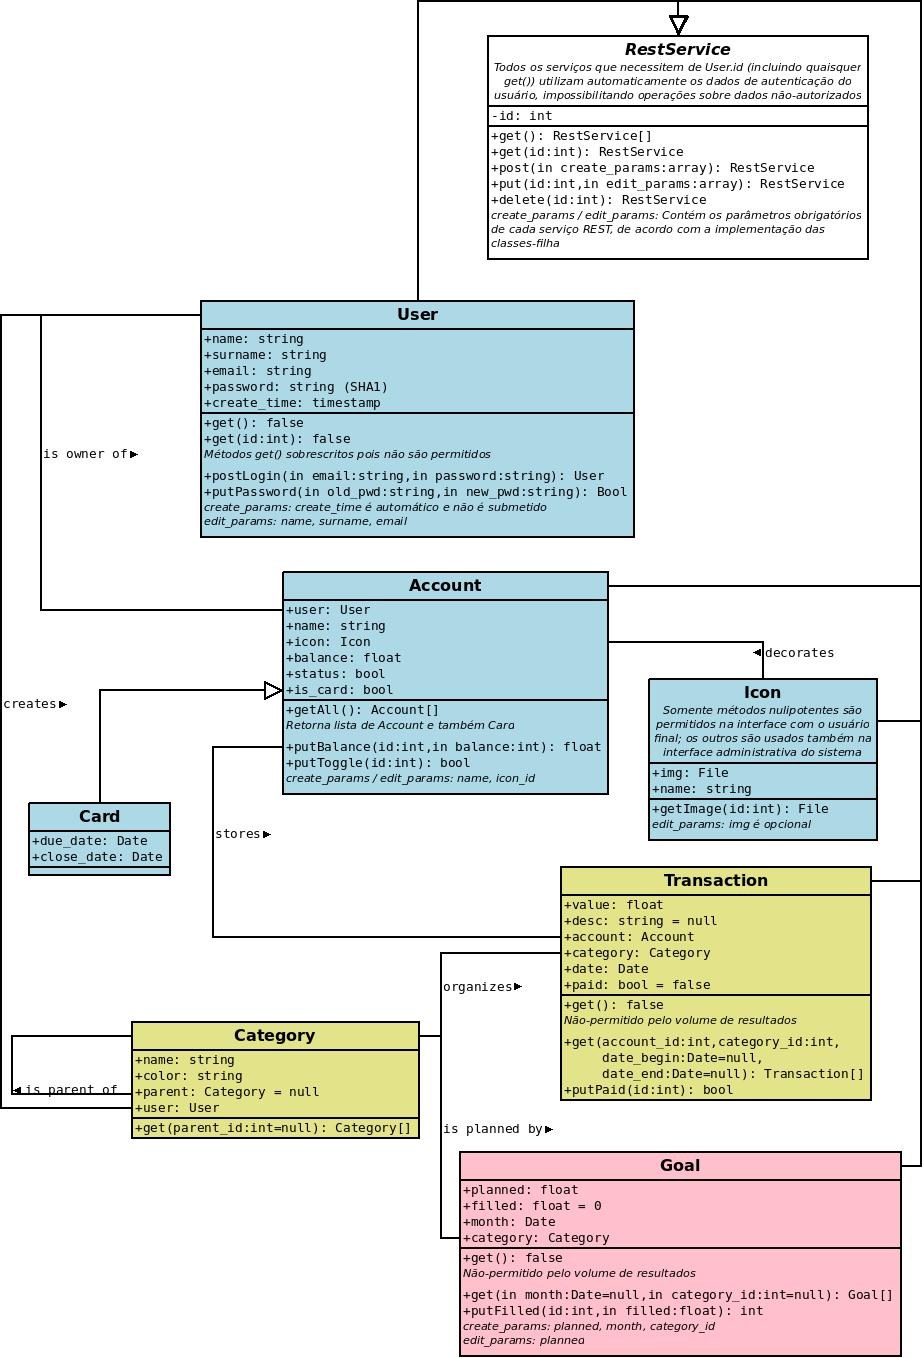
\includegraphics[scale=0.47]{diagramas/classes.jpg}
	\caption{Diagrama de Classes, demonstrando as principais classes do sistema REST}
\end{figure}

%%%%%%%%%%%%%%%%%%%%%%%%%%%%%%%%%%%%%%%%%%%%%%%%%%%%%%%%%%%%%%%%%%%%%%%%%%%%%%%%%%%%%%%%%
\begin{figure}
	\section{Modelo Conceitual de Dados}
	\label{sec:mod_dados}
	\centering
	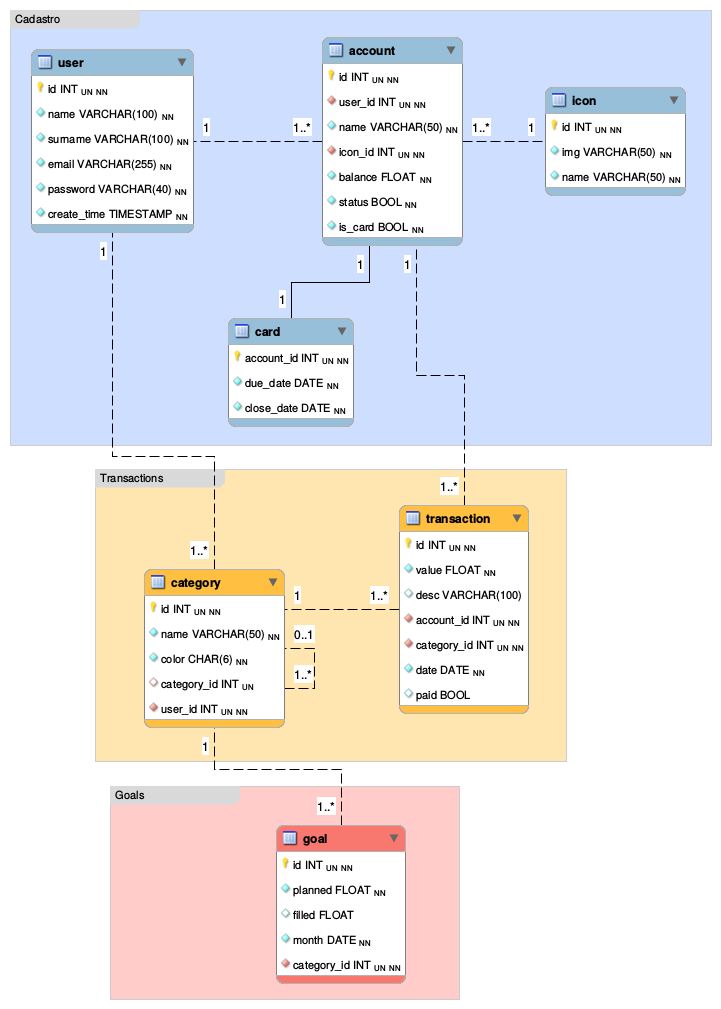
\includegraphics[scale=0.55]{diagramas/er.png}
	\caption{Diagrama de Entidade-Relacionamento, descrevendo o modelo de dados proposto para o projeto}

	%=======================================
	%
	% [TODO] Falta adicionar:
	% - transaction.paid [N bool=false]
	% - category.user+id [NN int]
	%
	%=======================================
	
\end{figure}

%%%%%%%%%%%%%%%%%%%%%%%%%%%%%%%%%%%%%%%%%%%%%%%%%%%%%%%%%%%%%%%%%%%%%%%%%%%%%%%%%%%%%%%%%
\printbibliography

\end{document}
